\chapter{技術構成}
基本的には、esaによりマークダウンを作成して、それをGitHubに保存して、GitHub Actionsを用いてhugoに出力して、Webサイトに公開する方法です。

ほぼほぼノーコードでできる構成になっているので、そこまで手間がかからずに作成をすることができます。

\begin{figure}[H]
  \centering
  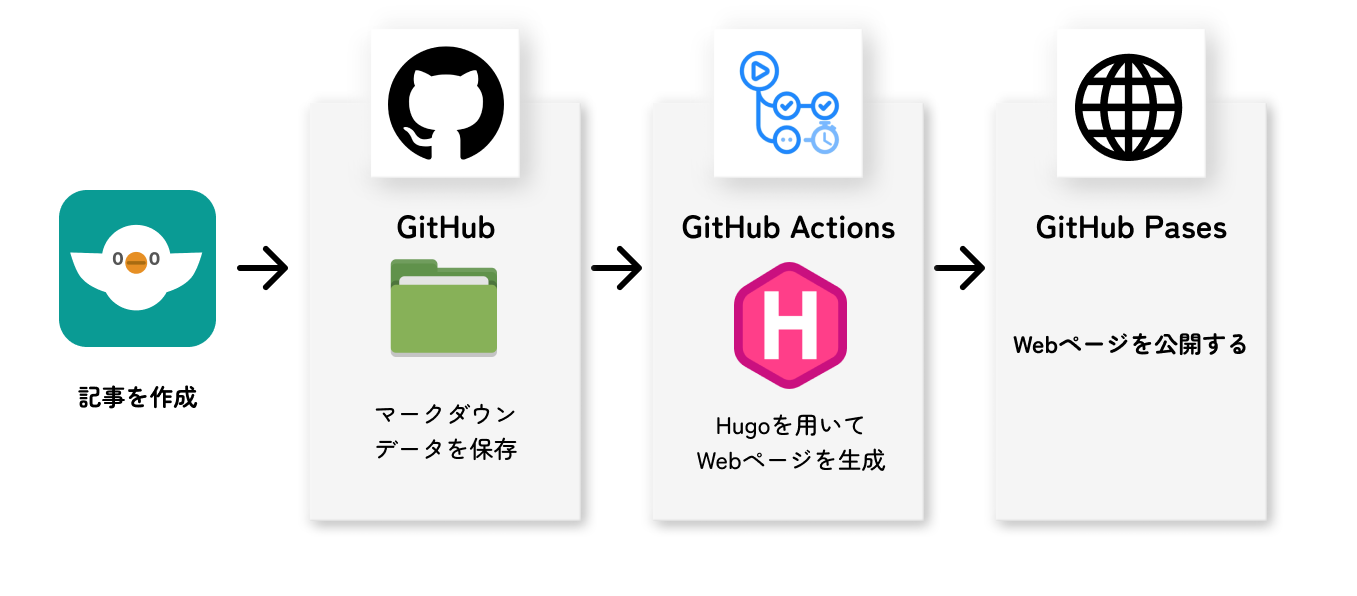
\includegraphics[width=14cm]{./image/02-chap4/flow.png}
  \caption{実際に用いた技術構成の図}
  \label{chap4-flow-image}
\end{figure}